\documentclass{article}\usepackage[]{graphicx}\usepackage[]{color}
% maxwidth is the original width if it is less than linewidth
% otherwise use linewidth (to make sure the graphics do not exceed the margin)
\makeatletter
\def\maxwidth{ %
  \ifdim\Gin@nat@width>\linewidth
    \linewidth
  \else
    \Gin@nat@width
  \fi
}
\makeatother

\definecolor{fgcolor}{rgb}{0.345, 0.345, 0.345}
\makeatletter
\@ifundefined{AddToHook}{}{\AddToHook{package/xcolor/after}{\definecolor{fgcolor}{rgb}{0.345, 0.345, 0.345}}}
\makeatother
\newcommand{\hlnum}[1]{\textcolor[rgb]{0.686,0.059,0.569}{#1}}%
\newcommand{\hlstr}[1]{\textcolor[rgb]{0.192,0.494,0.8}{#1}}%
\newcommand{\hlcom}[1]{\textcolor[rgb]{0.678,0.584,0.686}{\textit{#1}}}%
\newcommand{\hlopt}[1]{\textcolor[rgb]{0,0,0}{#1}}%
\newcommand{\hlstd}[1]{\textcolor[rgb]{0.345,0.345,0.345}{#1}}%
\newcommand{\hlkwa}[1]{\textcolor[rgb]{0.161,0.373,0.58}{\textbf{#1}}}%
\newcommand{\hlkwb}[1]{\textcolor[rgb]{0.69,0.353,0.396}{#1}}%
\newcommand{\hlkwc}[1]{\textcolor[rgb]{0.333,0.667,0.333}{#1}}%
\newcommand{\hlkwd}[1]{\textcolor[rgb]{0.737,0.353,0.396}{\textbf{#1}}}%
\let\hlipl\hlkwb

\usepackage{framed}
\makeatletter
\newenvironment{kframe}{%
 \def\at@end@of@kframe{}%
 \ifinner\ifhmode%
  \def\at@end@of@kframe{\end{minipage}}%
  \begin{minipage}{\columnwidth}%
 \fi\fi%
 \def\FrameCommand##1{\hskip\@totalleftmargin \hskip-\fboxsep
 \colorbox{shadecolor}{##1}\hskip-\fboxsep
     % There is no \\@totalrightmargin, so:
     \hskip-\linewidth \hskip-\@totalleftmargin \hskip\columnwidth}%
 \MakeFramed {\advance\hsize-\width
   \@totalleftmargin\z@ \linewidth\hsize
   \@setminipage}}%
 {\par\unskip\endMakeFramed%
 \at@end@of@kframe}
\makeatother

\definecolor{shadecolor}{rgb}{.97, .97, .97}
\definecolor{messagecolor}{rgb}{0, 0, 0}
\definecolor{warningcolor}{rgb}{1, 0, 1}
\definecolor{errorcolor}{rgb}{1, 0, 0}
\makeatletter
\@ifundefined{AddToHook}{}{\AddToHook{package/xcolor/after}{
\definecolor{shadecolor}{rgb}{.97, .97, .97}
\definecolor{messagecolor}{rgb}{0, 0, 0}
\definecolor{warningcolor}{rgb}{1, 0, 1}
\definecolor{errorcolor}{rgb}{1, 0, 0}
}}
\makeatother
\newenvironment{knitrout}{}{} % an empty environment to be redefined in TeX

\usepackage{alltt}


%%%%%%%%%%%%%%%%%%%%%%%%%%%%%%%%%%%%%%%%%
% Lachaise Assignment
% Structure Specification File
% Version 1.0 (26/6/2018)
%
% This template originates from:
% http://www.LaTeXTemplates.com
%
% Authors:
% Marion Lachaise & François Févotte
% Vel (vel@LaTeXTemplates.com)
%
% License:
% CC BY-NC-SA 3.0 (http://creativecommons.org/licenses/by-nc-sa/3.0/)
% 
%%%%%%%%%%%%%%%%%%%%%%%%%%%%%%%%%%%%%%%%%

%----------------------------------------------------------------------------------------
%	PACKAGES AND OTHER DOCUMENT CONFIGURATIONS
%----------------------------------------------------------------------------------------

\usepackage{amsmath,amsfonts,stmaryrd,amssymb} % Math packages

\usepackage[onehalfspacing]{setspace}

\usepackage{enumerate} % Custom item numbers for enumerations

\usepackage{amsopn}

\usepackage[ruled]{algorithm2e} % Algorithms

\usepackage[framemethod=tikz]{mdframed} % Allows defining custom boxed/framed environments

\usepackage{listings} % File listings, with syntax highlighting
\lstset{
	basicstyle=\ttfamily, % Typeset listings in monospace font
}
\usepackage[utf8]{inputenc}
\usepackage{array}
\usepackage{makecell}
\usepackage{placeins}
\usepackage{xcolor}
\usepackage{tikz}
\usetikzlibrary{matrix}
\usetikzlibrary{babel}

%----------------------------------------------------------------------------------------
%	DOCUMENT MARGINS
%----------------------------------------------------------------------------------------
\setlength{\parindent}{0pt}

\usepackage{geometry} % Required for adjusting page dimensions and margins

\geometry{
	paper=a4paper, % Paper size, change to letterpaper for US letter size
	top=1.5cm, % Top margin
	bottom=1.5cm, % Bottom margin
	left=1.5cm, % Left margin
	right=1.5cm, % Right margin
	headheight=10pt, % Header height
	footskip=1cm, % Space from the bottom margin to the baseline of the footer
	headsep=1.2cm, % Space from the top margin to the baseline of the header
	%showframe, % Uncomment to show how the type block is set on the page
}



%----------------------------------------------------------------------------------------
%	FONTS
%----------------------------------------------------------------------------------------

\usepackage[T1]{fontenc} % Output font encoding for international characters

\usepackage{XCharter} % Use the XCharter fonts

\usepackage{pgfplots}
\usepackage{tikz}
\usepgfplotslibrary{external}
%\tikzexternalize{main}

\newtheorem{theorem}{Theorem}[section]
\newtheorem{proposition}[theorem]{Proposition}
\newtheorem{defn}[theorem]{Definition}
\newtheorem{exmp}[theorem]{Example}
\newtheorem{corollary}[theorem]{Corollary}
\newtheorem{lemma}[theorem]{Lemma}
\newcommand*{\defeq}{\stackrel{\text{d}}{=}}
\newcommand*{\aseq}{\stackrel{\text{a.s.}}{=}}
%----------------------------------------------------------------------------------------
%	COMMAND LINE ENVIRONMENT
%----------------------------------------------------------------------------------------

% Usage:
% \begin{commandline}
%	\begin{verbatim}
%		$ ls
%		
%		Applications	Desktop	...
%	\end{verbatim}
% \end{commandline}

\mdfdefinestyle{commandline}{
	leftmargin=10pt,
	rightmargin=10pt,
	innerleftmargin=15pt,
	middlelinecolor=black!50!white,
	middlelinewidth=2pt,
	frametitlerule=false,
	backgroundcolor=black!5!white,
	frametitle={Command Line},
	frametitlefont={\normalfont\sffamily\color{white}\hspace{-1em}},
	frametitlebackgroundcolor=black!50!white,
	nobreak,
}

% Define a custom environment for command-line snapshots
\newenvironment{commandline}{
	\medskip
	\begin{mdframed}[style=commandline]
}{
	\end{mdframed}
	\medskip
}

%----------------------------------------------------------------------------------------
%	FILE CONTENTS ENVIRONMENT
%----------------------------------------------------------------------------------------

% Usage:
% \begin{file}[optional filename, defaults to "File"]
%	File contents, for example, with a listings environment
% \end{file}

\mdfdefinestyle{file}{
	innertopmargin=1.6\baselineskip,
	innerbottommargin=0.8\baselineskip,
	topline=false, bottomline=false,
	leftline=false, rightline=false,
	leftmargin=2cm,
	rightmargin=2cm,
	singleextra={%
		\draw[fill=black!10!white](P)++(0,-1.2em)rectangle(P-|O);
		\node[anchor=north west]
		at(P-|O){\ttfamily\mdfilename};
		%
		\def\l{3em}
		\draw(O-|P)++(-\l,0)--++(\l,\l)--(P)--(P-|O)--(O)--cycle;
		\draw(O-|P)++(-\l,0)--++(0,\l)--++(\l,0);
	},
	nobreak,
}

% Define a custom environment for file contents
\newenvironment{file}[1][File]{ % Set the default filename to "File"
	\medskip
	\newcommand{\mdfilename}{#1}
	\begin{mdframed}[style=file]
}{
	\end{mdframed}
	\medskip
}

%----------------------------------------------------------------------------------------
%	NUMBERED QUESTIONS ENVIRONMENT
%----------------------------------------------------------------------------------------

% Usage:
% \begin{question}[optional title]
%	Question contents
% \end{question}

\mdfdefinestyle{question}{
	innertopmargin=1.2\baselineskip,
	innerbottommargin=0.8\baselineskip,
	roundcorner=5pt,
	nobreak,
	singleextra={%
		\draw(P-|O)node[xshift=1em,anchor=west,fill=white,draw,rounded corners=5pt]{%
		Question \theQuestion\questionTitle};
	},
}

\newcounter{Question} % Stores the current question number that gets iterated with each new question

% Define a custom environment for numbered questions
\newenvironment{question}[1][\unskip]{
	\bigskip
	\stepcounter{Question}
	\newcommand{\questionTitle}{~#1}
	\begin{mdframed}[style=question]
}{
	\end{mdframed}
	\medskip
}

%----------------------------------------------------------------------------------------
%	WARNING TEXT ENVIRONMENT
%----------------------------------------------------------------------------------------

% Usage:
% \begin{warn}[optional title, defaults to "Warning:"]
%	Contents
% \end{warn}

\mdfdefinestyle{warning}{
	topline=false, bottomline=false,
	leftline=false, rightline=false,
	nobreak,
	singleextra={%
		\draw(P-|O)++(-0.5em,0)node(tmp1){};
		\draw(P-|O)++(0.5em,0)node(tmp2){};
		\fill[black,rotate around={45:(P-|O)}](tmp1)rectangle(tmp2);
		\node at(P-|O){\color{white}\scriptsize\bf !};
		\draw[very thick](P-|O)++(0,-1em)--(O);%--(O-|P);
	}
}

% Define a custom environment for warning text
\newenvironment{warn}[1][Warning:]{ % Set the default warning to "Warning:"
	\medskip
	\begin{mdframed}[style=warning]
		\noindent{\textbf{#1}}
}{
	\end{mdframed}
}

%----------------------------------------------------------------------------------------
%	INFORMATION ENVIRONMENT
%----------------------------------------------------------------------------------------

% Usage:
% \begin{info}[optional title, defaults to "Info:"]
% 	contents
% 	\end{info}

\mdfdefinestyle{info}{%
	topline=false, bottomline=false,
	leftline=false, rightline=false,
	nobreak,
	singleextra={%
		\fill[black](P-|O)circle[radius=0.4em];
		\node at(P-|O){\color{white}\scriptsize\bf i};
		\draw[very thick](P-|O)++(0,-0.8em)--(O);%--(O-|P);
	}
}

% Define a custom environment for information
\newenvironment{info}[1][Info:]{ % Set the default title to "Info:"
	\medskip
	\begin{mdframed}[style=info]
		\noindent{\textbf{#1}}
}{
	\end{mdframed}
}
\pgfplotsset{compat=1.18}

\title{STAT 6289-11 Causal Inference \\ Homework 1}

\author{Eunice Wu}
\date{\today}
\IfFileExists{upquote.sty}{\usepackage{upquote}}{}
\begin{document}


\raggedright
\maketitle






\section*{Problem 1} 
a) (2pt) Suppose $X$ and $Y$ have joint density $p(X, Y)$. How is $\mathbb{E}[Y \mid X]$ defined? (Write it out in terms of an integral and density function).  


\vspace*{0.5cm}
$\mathbb{E}[Y \mid X] = \int_Y y\cdot f_{Y|X}(y|x) \ dy = \int_Y y\cdot \dfrac{p(X, Y)}{f_X(x)} \ dy = \dfrac{1}{f_Y(x)}\int_Y y\cdot p(X, Y) \ dy$   
\vspace*{0.5cm}


b) (2pt) If $X$ and $Y$ were independent, what does $\mathbb{E}[X \mid Y]$ reduce to? (Show why this is.). 


\vspace*{0.5cm}
$\mathbb{E}[Y \mid X] = \int_Y y\cdot \dfrac{p(X, Y)}{f_X(x)} \ dy 
=  \int_Y y\cdot \dfrac{f_X(x) \cdot f_Y(y)}{f_X(x)} \ dy  
=  \int_Y y\cdot f_Y(y) \ dy  = \mathbb{E}[Y] $   
\vspace*{0.5cm}


c) (4pt) Draw random variables $X_{1}, X_{2}, \ldots, X_{N}$, all independently from the marginal density of $X$. Let $\bar{X}=\dfrac{1}{N} \sum_{i}^{N} X_{i}$. Is $\bar{X}$ unbiased for $\mathbb{E}[X]$ ? Prove it. (Do not just cite a theorem!)   


\vspace*{0.5cm}
The mean  $\bar{X}$ of a random sample is an unbiased estimate of the population moment $\mu = \mathbb{E}[X]$,
as $
\mathbb{E}(\bar{x})=\mathbb{E}\left(\sum \dfrac{X_{i}}{n}\right)=\dfrac{1}{n} \sum \mathbb{E}\left(X_{i}\right)=\dfrac{n}{n} \mu=\mu $   
\vspace{0.5cm}


d) (4pt) Derive the variance of $\bar{X}$. What happens to it as $N \rightarrow \infty$? 


\vspace{0.5cm}
$
\operatorname{Var}(\bar{X})=\operatorname{Var}\left(\sum \dfrac{X_{i}}{n}\right)=\dfrac{1}{n^{2}} \sum \operatorname{Var}\left(X_{i}\right)=\dfrac{n}{n^{2}} \sigma^{2}=\dfrac{\sigma^{2}}{n}
$  
When $N \rightarrow \infty$, $\operatorname{Var}(\bar{X}) \rightarrow \infty$   
\vspace*{0.5cm}

\section*{Problem 2}

Consider random variables $Y \in \mathbb{R}$ and $X \in \mathbb{R}^{\mathbb{P}}$, drawn from joint density $p(X, Y)$. You collect a sample of draws from this distribution, $\left\{\left(Y_{1}, X_{i}\right), \ldots,\left(Y_{N}, X_{N}\right)\right\}$.   
Let $\mathbf{X}$ be a $N \times(1+P)$ matrix, with row $i$ equal to $\left[1 X_{i}^{\top}\right]$ (i.e., there is an intercept and then a column for each "covariate"). Consider an OLS model, $Y=\mathbf{X} \beta+\epsilon$, where $\mathbb{E}[\epsilon \mid X]=0$. 


a) (4pt) Using matrix notation at each step, derive the ordinary least squares estimator for $\beta$ :

$$
\hat{\beta}=\underset{\beta \in \mathbb{R}^{P+1}}{\operatorname{argmin}}(\mathbf{Y}-\mathbf{X} \beta)^{\top}(\mathbf{Y}-\mathbf{X} \beta)
$$


\vspace*{0.5cm}
$$
\left[\begin{array}{c}
Y_{1} \\
Y_{2} \\
\vdots \\
\vdots \\
Y_{N}
\end{array}\right]_{N \times 1}=\left[\begin{array}{ccccc}
1 & X_{11} & X_{21} & \ldots & X_{p 1} \\
1 & X_{12} & X_{22} & \ldots & X_{p 2} \\
\vdots & \vdots & \vdots & \ldots & \vdots \\
\vdots & \vdots & \vdots & \ldots & \vdots \\
1 & X_{1 n} & X_{2 n} & \ldots & X_{p N}
\end{array}\right]_{N \times (p+1)}\left[\begin{array}{c}
\beta_{0} \\
\beta_{2} \\
\vdots \\
\beta_{p}
\end{array}\right]_{(p+1) \times 1}+\left[\begin{array}{c}
\varepsilon_{1} \\
\varepsilon_{2} \\
\vdots \\
\vdots \\
\varepsilon_{N}
\end{array}\right]_{N \times 1}
$$


$$
\begin{aligned}
\varepsilon^{T} \varepsilon &=(\mathbf{Y}-\mathbf{X} \hat{\beta})^{T}(\mathbf{Y}-\mathbf{X} \hat{\beta}) \\
&=\mathbf{Y}^{T} \mathbf{Y}-\hat{\beta}^{T} \mathbf{X}^{T} \mathbf{Y}-\mathbf{Y}^{T} \mathbf{X} \hat{\beta}+\hat{\beta}^{T} \mathbf{X}^{T} \mathbf{X} \hat{\beta} \\
&=\mathbf{Y}^{T} \mathbf{Y}-2 \hat{\beta}^{T} \mathbf{X}^{T} \mathbf{Y}+\hat{\beta}^{T} \mathbf{X}^{\prime} \mathbf{X} \hat{\beta}
\end{aligned} 
$$


$$
\begin{aligned}
&\dfrac{\partial \varepsilon^{T} \varepsilon}{\partial \hat{\beta}}=-2 \mathbf{X}^{\prime} \mathbf{Y}+2 \mathbf{X}^{\prime} \mathbf{X} \hat{\beta}=0 \quad
\dfrac{\partial^2 \varepsilon^{T} \varepsilon}{\partial \hat{\beta}^2}= 2 \mathbf{X}^{T} \mathbf{X} >0
\\
\Rightarrow 
&\left(\mathbf{X}^{T} \mathbf{X}\right) \hat{\beta}=\mathbf{X}^{T} \mathbf{Y}
\\
&\left(\mathbf{X}^{T} \mathbf{X}\right)^{-1}\left(\mathbf{X}^{T} \mathbf{X}\right) \hat{\beta}=\left(\mathbf{X}^{T} X\right)^{-1} \mathbf{X}^{T}\mathbf{Y}
\\
&I \hat{\beta} =\left(\mathbf{X}^{T} \mathbf{X}\right)^{-1} \mathbf{X}^{T} \mathbf{Y} \\
&\hat{\beta} =\left(\mathbf{X}^{T} \mathbf{X}\right)^{-1} \mathbf{X}^{T} \mathbf{Y}
\end{aligned}
$$
\vspace*{0.5cm}


b) (5pt) Show $R$ code that would achieve the following:

i. Construct a matrix $X$ to represent $\mathbf{X}$ in the above, with $N=100$, one column of ones, and two columns of randomly drawn numbers (from any distribution you like).

\begin{knitrout}
\definecolor{shadecolor}{rgb}{0.969, 0.969, 0.969}\color{fgcolor}\begin{kframe}
\begin{alltt}
\hlstd{N} \hlkwb{=} \hlnum{100}
\hlstd{X} \hlkwb{<-} \hlkwd{cbind}\hlstd{(}\hlkwd{matrix}\hlstd{(}\hlnum{1}\hlopt{:}\hlnum{1}\hlstd{,} \hlkwc{ncol} \hlstd{=} \hlnum{1}\hlstd{,} \hlkwc{nrow} \hlstd{= N),}  \hlkwd{matrix}\hlstd{(}\hlkwd{rpois}\hlstd{(N,} \hlnum{5}\hlstd{),} \hlkwc{ncol} \hlstd{=} \hlnum{1}\hlstd{),}
           \hlkwd{matrix}\hlstd{(}\hlkwd{rpois}\hlstd{(N,} \hlnum{10}\hlstd{),} \hlkwc{ncol} \hlstd{=} \hlnum{1}\hlstd{))}
\hlkwd{head}\hlstd{(X)}
\end{alltt}
\begin{verbatim}
##      [,1] [,2] [,3]
## [1,]    1    6   13
## [2,]    1    5   14
## [3,]    1    4    4
## [4,]    1    7    8
## [5,]    1    1   12
## [6,]    1    4   13
\end{verbatim}
\end{kframe}
\end{knitrout}
\vspace*{0.5cm}


ii. Using $\beta=\left[\begin{array}{lll}1 & 2 & 3\end{array}\right]^{\top}$, compute vector $Y$ equal to $X \beta+\epsilon$, where $\epsilon$ is drawn from a standard normal distribution.

\begin{knitrout}
\definecolor{shadecolor}{rgb}{0.969, 0.969, 0.969}\color{fgcolor}\begin{kframe}
\begin{alltt}
\hlstd{beta} \hlkwb{=} \hlkwd{c}\hlstd{(}\hlnum{1}\hlstd{,}\hlnum{2}\hlstd{,}\hlnum{3}\hlstd{)}
\hlstd{epsilon} \hlkwb{=} \hlkwd{matrix}\hlstd{(}\hlkwd{rnorm}\hlstd{(N,} \hlkwc{mean}\hlstd{=}\hlnum{0}\hlstd{,} \hlkwc{sd}\hlstd{=}\hlnum{1}\hlstd{),} \hlkwc{ncol} \hlstd{=} \hlnum{1}\hlstd{)}
\hlstd{beta}
\end{alltt}
\begin{verbatim}
## [1] 1 2 3
\end{verbatim}
\begin{alltt}
\hlkwd{head}\hlstd{(epsilon)}
\end{alltt}
\begin{verbatim}
##            [,1]
## [1,]  0.3260207
## [2,]  0.0932062
## [3,] -0.2524867
## [4,] -0.2877227
## [5,]  0.6339740
## [6,] -0.6630345
\end{verbatim}
\begin{alltt}
\hlstd{Y} \hlkwb{=} \hlstd{X} \hlopt \hlstd{beta} \hlopt{+} \hlstd{epsilon}
\hlkwd{head}\hlstd{(Y)}
\end{alltt}
\begin{verbatim}
##          [,1]
## [1,] 52.32602
## [2,] 53.09321
## [3,] 20.74751
## [4,] 38.71228
## [5,] 39.63397
## [6,] 47.33697
\end{verbatim}
\end{kframe}
\end{knitrout}

iii. Compute $\left(X^{\top} X\right)^{-1}\left(X^{\top} Y\right)$. Use the solve function in $\mathrm{R}$.

\begin{knitrout}
\definecolor{shadecolor}{rgb}{0.969, 0.969, 0.969}\color{fgcolor}\begin{kframe}
\begin{alltt}
\hlstd{beta_est} \hlkwb{=} \hlkwd{solve}\hlstd{(}\hlkwd{t}\hlstd{(X)} \hlopt \hlstd{X)}  \hlopt \hlkwd{t}\hlstd{(X)}  \hlopt \hlstd{Y}
\hlstd{beta_est}
\end{alltt}
\begin{verbatim}
##           [,1]
## [1,] 0.6751192
## [2,] 1.9567181
## [3,] 3.0473170
\end{verbatim}
\end{kframe}
\end{knitrout}

iv. Compare the result to the coefficients obtained using lm with the data you have constructed.

\begin{knitrout}
\definecolor{shadecolor}{rgb}{0.969, 0.969, 0.969}\color{fgcolor}\begin{kframe}
\begin{alltt}
\hlstd{coeff_lm} \hlkwb{<-} \hlkwd{lm}\hlstd{(Y} \hlopt{~} \hlstd{X[,}\hlnum{2}\hlstd{]}\hlopt{+}\hlstd{X[,}\hlnum{3}\hlstd{])}
\hlkwd{summary}\hlstd{(coeff_lm)}
\end{alltt}
\begin{verbatim}
## 
## Call:
## lm(formula = Y ~ X[, 2] + X[, 3])
## 
## Residuals:
##      Min       1Q   Median       3Q      Max 
## -2.15919 -0.54278  0.04758  0.52232  2.39986 
## 
## Coefficients:
##             Estimate Std. Error t value Pr(>|t|)    
## (Intercept)  0.67512    0.37629   1.794   0.0759 .  
## X[, 2]       1.95672    0.04659  42.001   <2e-16 ***
## X[, 3]       3.04732    0.03161  96.401   <2e-16 ***
## ---
## Signif. codes:  0 '***' 0.001 '**' 0.01 '*' 0.05 '.' 0.1 ' ' 1
## 
## Residual standard error: 0.9595 on 97 degrees of freedom
## Multiple R-squared:  0.9922,	Adjusted R-squared:  0.992 
## F-statistic:  6136 on 2 and 97 DF,  p-value: < 2.2e-16
\end{verbatim}
\end{kframe}
\end{knitrout}

c) (5pt) Prove the unbiasedness of $\hat{\beta}$ for $\beta$.

\vspace*{0.5cm}
% $Y_i = \beta_0 + \beta_1X_i + \varepsilon_i$
% 
% $\mathbb{E}(\varepsilon_i) = 0$
% 
% $\mathbb{E}(Y_i) = \mathbb{E}( \beta_0 + \beta_1X_i + \varepsilon_i) 
% = \mathbb{E}(\beta_0) + \mathbb{E} (\beta_1X_i) + \mathbb{E}(\varepsilon_i)$
% 
% $\mathbb{E}(\bar{Y}) = \mathbb{E}(\dfrac{1}{n} \sum_{i=1}^n{Y_i}) 
% = \dfrac{1}{n} \sum_{i=1}^{n} \mathbb{E}(Y_i) 
% = \dfrac{1}{n} \sum_{i=1}^{n} \beta_0 + \beta_1X_i 
% = \dfrac{n\beta_0}{n} + \beta_1 \cdot \dfrac{\sum_{i=1}^{n}X_i}{n}
% = \beta_0 + \beta_1 \bar{X} $
% 
% $\mathbb{E}(\hat{\beta_1}) = \mathbb{E} \left(\dfrac{\sum_{i=1}^{n} (X_i - \bar{X})Y_i}{\sum_{i=1}^{n}(X_i - \bar{X})X_i}   \right) 
% = \dfrac{\sum_{i=1}^{n} (X_i - \bar{X})\mathbb{E}(Y_i)}{\sum_{i=1}^{n}(X_i - \bar{X})X_i}   
% =  \dfrac{\sum_{i=1}^{n} (X_i - \bar{X})(\beta_0 + \beta_1X_i)}{\sum_{i=1}^{n}(X_i - \bar{X})X_i}  
% = \dfrac{\beta_0 \cdot \sum_{i=1}^{n} (X_i - \bar{X})}{\sum_{i=1}^{n}(X_i - \bar{X})X_i} + \dfrac{\beta_1 \cdot \sum_{i=1}^{n} (X_i - \bar{X})X_i}{\sum_{i=1}^{n}(X_i - \bar{X})X_i} 
% = 0+\beta_1
% = \beta_1
% $
% 
% $
% \mathbb{E}(\hat{\beta_0}) = \mathbb{E}(\bar{Y} - \hat{\beta_1} \cdot \bar{X}) = \mathbb{E}(\bar{Y}) - \bar{X}\mathbb{E}(\hat{\beta_1}) = \beta_0 + \beta_1\bar{X} - \beta_1\bar{X} = \beta_0
% $
% 
% So $\hat{\beta}$ is an unbiased estimator of $\beta$. 
% \vspace*{0.5cm}

With Matrix notation: 

$\hat{\beta}=\left(\mathbf{X}^{T} \mathbf{X}\right)^{-1} \mathbf{X}^{T} \mathbf{Y} =\left(\mathbf{X}^{T} \mathbf{X}\right)^{-1} \mathbf{X}^{T}(\mathbf{X} \beta+\varepsilon) =\beta+\left(\mathbf{X}^{T} \mathbf{X}\right)^{-1} \mathbf{X}^{T} \varepsilon$ 

And $\left(\mathbf{X}^{T} \mathbf{X}\right)^{-1} \mathbf{X}^{T} \mathbf{X}=I$. 

So 
$\mathbb{E}[\hat{\beta}] =\mathbb{E}[\beta]+\mathbb{E}\left[\left(\mathbf{X}^{T} \mathbf{X}\right)^{-1} \mathbf{X}^{T} \varepsilon\right] 
=\beta+\left(\mathbf{X}^{T} \mathbf{X}\right)^{-1} \mathbf{X}^{T} \mathbb{E}[\varepsilon]$


$\mathbb{E}[\varepsilon]=0$. So


$
\mathbb{E}(\hat{\beta}) 
=\mathbb{E}(\beta)+\mathbb{E}\left[\left(\mathbf{X}^{T} \mathbf{X} \right)^{-1} \mathbf{X}^{T} \varepsilon \right] 
=\beta+\left(\mathbf{X}^{T} \mathbf{X}\right)^{-1} \mathbb{E}\left[\mathbf{X}^{T} \varepsilon\right]
$


As $\mathbb{E}\left(\mathbf{X}^{T} \varepsilon\right)=0$, $\mathbb{E}(\hat{\beta})  = \beta$
\vspace*{0.5cm}


d) (5pt) Compute the variance, with $\mathbf{X}$ taken as fixed (not random), i.e. $\mathbb{V}[\hat{\beta} \mid \mathbf{X}]$, again sticking with matrix notation. You may assume $\mathbb{E}\left[\epsilon \epsilon^{\top} \mid \mathbf{X}\right]=\sigma^{2} I_{N}$, where $I_{N}$ is the $N \times N$ identity matrix.

\vspace*{0.5cm}
$
\begin{aligned}
\mathbb{E}\left[(\hat{\beta}-\beta)(\hat{\beta}-\beta)^{T}\right]  &=\mathbb{E}\left[\left(\left(\mathbf{X}^{T} \mathbf{X}\right)^{-1} \mathbf{X}^{T} \varepsilon\right)\left(\left(\mathbf{X}^{T} \mathbf{X}\right)^{-1} \mathbf{X}^{T} \varepsilon\right)^{T}\right]  \\ &=\mathbb{E}\left[\left(\mathbf{X}^{T} \mathbf{X}\right)^{-1} \mathbf{X}^{T} \varepsilon \varepsilon^{T} \mathbf{X}\left(\mathbf{X}^{T} \mathbf{X}\right)^{-1}\right] \\
&= \left(\mathbf{X}^{T} \mathbf{X}\right)^{-1} \mathbf{X}^{T} \mathbb{E}\left[\varepsilon \varepsilon ^{T}\right] \mathbf{X}\left(\mathbf{X}^{T} \mathbf{X}\right)^{-1} \\
&=\left(\mathbf{X}^{T} \mathbf{X}\right)^{-1} \mathbf{X}^{T}\left(\sigma^{2} I\right) \mathbf{X}\left(\mathbf{X}^{T} \mathbf{X}\right)^{-1} \\
&=\sigma^{2} I\left(\mathbf{X}^{T} \mathbf{X}\right)^{-1} \mathbf{X}^{T} \mathbf{X}\left(\mathbf{X}^{T} \mathbf{X}\right)^{-1}  \\
&=\sigma^{2}\left(\mathbf{X}^{T} \mathbf{X}\right)^{-1}
\end{aligned}
$

Therefore, 

$\operatorname{Var}(\hat{\beta}) = 
\mathbb{E}\left[(\hat{\beta}-\beta)(\hat{\beta}-\beta)^{T}\right] 
= \left[\begin{array}{cccc}
\operatorname{var}\left(\hat{\beta}_{1}\right) & \operatorname{cov}\left(\hat{\beta}_{1}, \hat{\beta}_{2}\right) & \ldots & \operatorname{cov}\left(\hat{\beta}_{1}, \hat{\beta}_{k}\right) \\
\operatorname{cov}\left(\hat{\beta}_{2}, \hat{\beta}_{1}\right) & \operatorname{var}\left(\hat{\beta}_{2}\right) & \ldots & \operatorname{cov}\left(\hat{\beta}_{2}, \hat{\beta}_{k}\right) \\
\vdots & \vdots & \vdots & \vdots \\
\operatorname{cov}\left(\hat{\beta}_{k}, \hat{\beta}_{1}\right) & \operatorname{cov}\left(\hat{\beta}_{k}, \hat{\beta}_{2}\right) & \ldots & \operatorname{var}\left(\hat{\beta}_{k}\right)
\end{array}\right]
$
\vspace*{0.5cm}

e) (2pt) What meaning would you give to the matrix $\mathbb{E}\left[\epsilon \epsilon^{\top} \mid \mathbf{X}\right]$ ? Give an intuitive explanation of what the assumption that this matrix equals $\sigma^{2} I$ implies.

\vspace*{0.5cm}
The variance of $\varepsilon_i$ is the same for all $X_i$ and $\varepsilon_i$'s are independent. 
\vspace*{0.5cm}


\section*{Problem 3}

Which of the following statements are true or false? For credit, explain your choice briefly

a) (3pt) If there is perfect collinearity, the OLS estimator will give biased and inconsistent estimates.

\vspace*{0.5cm}
Not true. The coefficients on the collinear terms might have infinite variance if the collinearity is extreme while the estimator remains unbiased. 
\vspace*{0.5cm}

b) (3pt) A very large p-value for the estimated coefficient for an explanatory variable provides strong evidence that the variable has zero effect on the outcome.

\vspace*{0.5cm}
Not true. If the p-value is larger than the confidence level during F-test, we rejected the null hypothesis and it can be concluded that there is at least one coefficient is not zero. 
\vspace*{0.5cm}


c) (3pt) If an estimator is unbiased it is also consistent.

\vspace*{0.5cm}
Not true. 
\vspace*{0.5cm}

d) (3pt) You have a model $Y=X^{\top} \beta+\epsilon$, and you fit it by OLS. If the OLS residuals are uncorrelated with $X$, our estimate of $\beta$ are unbiased. 

\vspace*{0.5cm}
True. 
$
\mathbb{E}(\hat{\beta}) 
=\beta+\left(\mathbf{X}^{T} \mathbf{X}\right)^{-1} \mathbb{E}\left[\mathbf{X}^{T} \varepsilon\right]
$
If $\mathbb{E}\left(\mathbf{X}^{T} \varepsilon\right)= \mathbb{E}(\varepsilon) = 0, \mathbb{E}(\hat{\beta})  = \beta$
\vspace*{0.5cm}



\section*{Problem 4}

Suppose $X_{1} \sim N(5,2)$ and $X_{2} \sim \exp (\lambda=1)$ (where $\exp$ indicates the exponential distribution). In $\mathrm{R}$, construct two vectors, $\mathrm{X1}$ with 10000 draws from the same distribution as $X_{1}$, and $\mathrm{X2}$ with 10000 draws from the same distribution as $X_{2}$.

We will take sub-samples from these two variables to evaluate the coverage probability of $95 \%$ confidence intervals using different types of data and different sample sizes.

(a) (4pt) Describe the distribution of $\mathrm{X1}$ and $\mathrm{X2}$ using histograms. Mark the true (population) expectation on your plot using a line.

\vspace*{0.5cm}
\begin{knitrout}
\definecolor{shadecolor}{rgb}{0.969, 0.969, 0.969}\color{fgcolor}\begin{kframe}
\begin{alltt}
\hlstd{X1} \hlkwb{<-} \hlkwd{matrix}\hlstd{(}\hlkwd{rnorm}\hlstd{(}\hlnum{10000}\hlstd{,} \hlkwc{mean} \hlstd{=} \hlnum{5}\hlstd{,} \hlkwc{sd} \hlstd{=} \hlnum{1}\hlstd{),}\hlkwc{ncol} \hlstd{=} \hlnum{1}\hlstd{)}
\hlstd{X2} \hlkwb{<-} \hlkwd{matrix}\hlstd{(}\hlkwd{rpois}\hlstd{(}\hlnum{10000}\hlstd{,} \hlnum{1}\hlstd{),}\hlkwc{ncol} \hlstd{=} \hlnum{1}\hlstd{)}
\hlkwd{head}\hlstd{(X1)}
\end{alltt}
\begin{verbatim}
##          [,1]
## [1,] 5.257544
## [2,] 4.818645
## [3,] 6.778251
## [4,] 3.542059
## [5,] 4.783530
## [6,] 5.105978
\end{verbatim}
\begin{alltt}
\hlkwd{head}\hlstd{(X2)}
\end{alltt}
\begin{verbatim}
##      [,1]
## [1,]    1
## [2,]    0
## [3,]    0
## [4,]    2
## [5,]    2
## [6,]    3
\end{verbatim}
\end{kframe}
\end{knitrout}

\begin{knitrout}
\definecolor{shadecolor}{rgb}{0.969, 0.969, 0.969}\color{fgcolor}\begin{kframe}
\begin{alltt}
\hlkwd{hist}\hlstd{(X1)}
\hlkwd{abline}\hlstd{(}\hlkwc{v} \hlstd{=} \hlkwd{mean}\hlstd{(X1),} \hlkwc{col} \hlstd{=} \hlstr{"yellow"}\hlstd{,} \hlkwc{lwd} \hlstd{=} \hlnum{2}\hlstd{)}
\end{alltt}
\end{kframe}
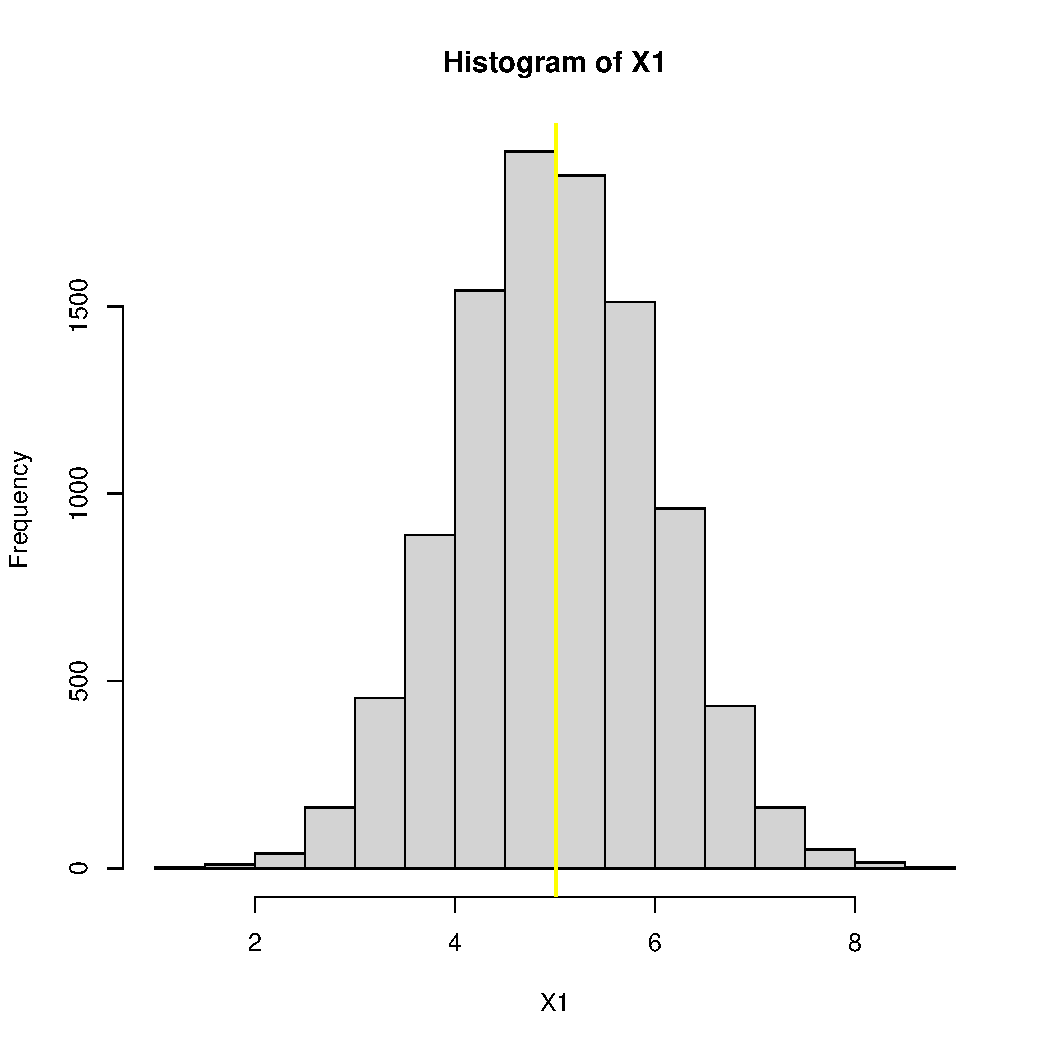
\includegraphics[width=\maxwidth]{figure/unnamed-chunk-7-1} 
\end{knitrout}

\begin{knitrout}
\definecolor{shadecolor}{rgb}{0.969, 0.969, 0.969}\color{fgcolor}\begin{kframe}
\begin{alltt}
\hlkwd{hist}\hlstd{(X2)}
\hlkwd{abline}\hlstd{(}\hlkwc{v} \hlstd{=} \hlkwd{mean}\hlstd{(X2),} \hlkwc{col} \hlstd{=} \hlstr{"blue"}\hlstd{,} \hlkwc{lwd} \hlstd{=} \hlnum{2}\hlstd{)}
\end{alltt}
\end{kframe}
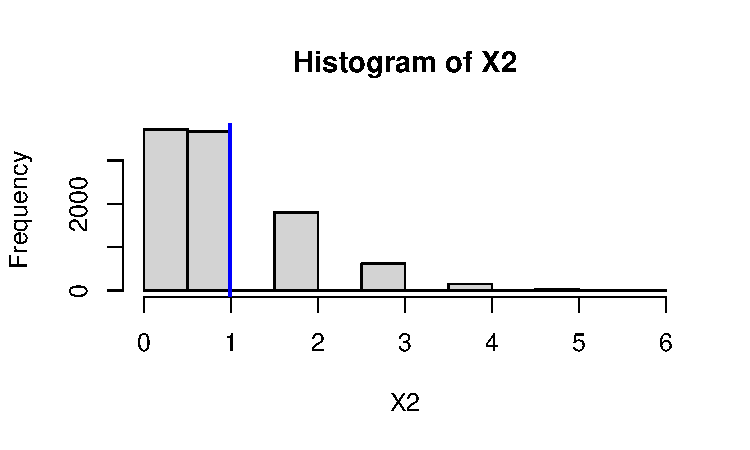
\includegraphics[width=\maxwidth]{figure/unnamed-chunk-8-1} 
\end{knitrout}

\vspace*{0.5cm}

(b) $(4 \mathrm{pts})$ Consider for a moment the random variables $\bar{X}_{1}$ and $\bar{X}_{2}$, representing sample means. Using math (not $R$ ), give solutions for:

- $\mathbb{E}\left[\bar{X}_{1}\right]$ ?

- $\mathbb{E}\left[\bar{X}_{2}\right]$ ?

- $\operatorname{Var}\left(\bar{X}_{1}\right)$ ?

- $\operatorname{Var}\left(\bar{X}_{2}\right)$ ?

\vspace*{0.5cm}
$\mathbb{E}\left[\bar{X}_{1}\right] = 5$

$\mathbb{E}\left[\bar{X}_{2}\right] = 1$

$\operatorname{Var}\left(\bar{X}_{1}\right) = 2$ 

$\operatorname{Var}\left(\bar{X}_{2}\right) = 1$ 
\vspace*{0.5cm}

(c) (4pts). Now, for $X_{1}$, draw 5000 sub-samples each of size $N=6$. Get the sample mean and compute the $95 \%$ confidence interval each time. What portion of the confidence intervals you computed include the true expectation? Repeat this for $X_{2}$.

\begin{knitrout}
\definecolor{shadecolor}{rgb}{0.969, 0.969, 0.969}\color{fgcolor}\begin{kframe}
\begin{alltt}
\hlstd{X1_sub_sample} \hlkwb{<-} \hlkwd{matrix}\hlstd{(}\hlkwd{sample}\hlstd{(X1,} \hlkwc{size} \hlstd{=} \hlnum{5000} \hlopt{*}\hlnum{6}\hlstd{,} \hlkwc{replace} \hlstd{=} \hlnum{TRUE}\hlstd{),}\hlnum{6}\hlstd{,} \hlnum{5000}\hlstd{)}

\hlkwd{head}\hlstd{(X1_sub_sample,}\hlnum{5}\hlopt{:}\hlnum{6}\hlstd{)}
\end{alltt}
\begin{verbatim}
##          [,1]     [,2]     [,3]     [,4]     [,5]     [,6]
## [1,] 3.085447 5.183113 5.758012 4.273961 5.115787 5.731389
## [2,] 5.329938 3.545789 5.154577 5.053304 3.081665 4.560495
## [3,] 4.433019 7.033668 5.493081 3.634116 5.217159 6.808585
## [4,] 5.897117 5.747834 4.940110 5.033851 3.941513 4.967928
## [5,] 5.856407 5.832355 4.256276 4.470993 5.094903 4.124827
\end{verbatim}
\begin{alltt}
\hlstd{X1_sub_sample_mean} \hlkwb{=} \hlkwd{apply}\hlstd{(X1_sub_sample,} \hlnum{2}\hlstd{, mean)}

\hlcom{#head(X1_sub_sample_mean)}

\hlstd{X1_sub_sample_ci} \hlkwb{=} \hlkwd{apply}\hlstd{(X1_sub_sample,} \hlnum{2}\hlstd{,} \hlkwa{function}\hlstd{(}\hlkwc{x}\hlstd{)} \hlkwd{ci}\hlstd{(x))}

\hlkwd{head}\hlstd{(X1_sub_sample_ci,}\hlnum{5}\hlopt{:}\hlnum{6}\hlstd{)}
\end{alltt}
\begin{verbatim}
##                 [,1]     [,2]      [,3]      [,4]      [,5]      [,6]
## Estimate   5.0559698 5.506918 5.1162317 4.7669467 4.7436136 5.0104831
## CI lower   3.8917212 4.311981 4.5757271 3.8715399 3.6432567 3.8567714
## CI upper   6.2202184 6.701856 5.6567364 5.6623536 5.8439705 6.1641948
## Std. Error 0.4529125 0.464851 0.2102655 0.3483285 0.4280575 0.4488134
\end{verbatim}
\begin{alltt}
\hlkwd{sum}\hlstd{(}\hlkwd{apply}\hlstd{(X1_sub_sample_ci,} \hlnum{2}\hlstd{,} \hlkwa{function}\hlstd{(}\hlkwc{x}\hlstd{)\{}\hlkwd{ifelse}\hlstd{(x[}\hlnum{2}\hlstd{]} \hlopt{<} \hlnum{5} \hlopt{&} \hlstd{x[}\hlnum{3}\hlstd{]} \hlopt{>} \hlnum{5}\hlstd{,}
                                                  \hlnum{TRUE}\hlstd{,} \hlnum{FALSE}\hlstd{)\}))}
\end{alltt}
\begin{verbatim}
## [1] 4752
\end{verbatim}
\end{kframe}
\end{knitrout}


\begin{knitrout}
\definecolor{shadecolor}{rgb}{0.969, 0.969, 0.969}\color{fgcolor}\begin{kframe}
\begin{alltt}
\hlstd{X2_sub_sample} \hlkwb{<-} \hlkwd{matrix}\hlstd{(}\hlkwd{sample}\hlstd{(X2,} \hlkwc{size} \hlstd{=} \hlnum{5000} \hlopt{*}\hlnum{6}\hlstd{,} \hlkwc{replace} \hlstd{=} \hlnum{TRUE}\hlstd{),}\hlnum{6}\hlstd{,} \hlnum{5000}\hlstd{)}

\hlkwd{head}\hlstd{(X2_sub_sample,}\hlnum{5}\hlopt{:}\hlnum{6}\hlstd{)}
\end{alltt}
\begin{verbatim}
##      [,1] [,2] [,3] [,4] [,5] [,6]
## [1,]    0    1    2    0    1    1
## [2,]    1    2    1    0    1    2
## [3,]    2    0    1    1    0    0
## [4,]    0    2    0    3    0    1
## [5,]    1    1    1    0    0    2
\end{verbatim}
\begin{alltt}
\hlstd{X2_sub_sample_mean} \hlkwb{=} \hlkwd{apply}\hlstd{(X2_sub_sample,} \hlnum{2}\hlstd{, mean)}

\hlstd{X2_sub_sample_ci} \hlkwb{=} \hlkwd{apply}\hlstd{(X2_sub_sample,} \hlnum{2}\hlstd{,} \hlkwa{function}\hlstd{(}\hlkwc{x}\hlstd{)} \hlkwd{ci}\hlstd{(x))}

\hlkwd{head}\hlstd{(X2_sub_sample_ci,}\hlnum{5}\hlopt{:}\hlnum{6}\hlstd{)}
\end{alltt}
\begin{verbatim}
##                  [,1]       [,2]      [,3]       [,4]        [,5]      [,6]
## Estimate   0.83333333 1.00000000 1.0000000  0.8333333  0.50000000 1.1666667
## CI lower   0.04334688 0.06135623 0.3362786 -0.3935044 -0.07479957 0.3766802
## CI upper   1.62331978 1.93864377 1.6637214  2.0601710  1.07479957 1.9566531
## Std. Error 0.30731815 0.36514837 0.2581989  0.4772607  0.22360680 0.3073181
\end{verbatim}
\begin{alltt}
\hlkwd{sum}\hlstd{(}\hlkwd{apply}\hlstd{(X2_sub_sample_ci,} \hlnum{2}\hlstd{,} \hlkwa{function}\hlstd{(}\hlkwc{x}\hlstd{)\{}\hlkwd{ifelse}\hlstd{(x[}\hlnum{2}\hlstd{]} \hlopt{<} \hlnum{1} \hlopt{&} \hlstd{x[}\hlnum{3}\hlstd{]} \hlopt{>} \hlnum{1}\hlstd{,}
                                                  \hlnum{TRUE}\hlstd{,} \hlnum{FALSE}\hlstd{)\}))}
\end{alltt}
\begin{verbatim}
## [1] 4652
\end{verbatim}
\end{kframe}
\end{knitrout}


(d) (4pt) Repeat (c) for samples of size 6, 20, 50, and 500. Report the coverage probability for each of your eight simulations in a table. How do your results change? What differences do you see between X1 and X2?

\begin{knitrout}
\definecolor{shadecolor}{rgb}{0.969, 0.969, 0.969}\color{fgcolor}\begin{kframe}
\begin{alltt}
\hlcom{#X1 sampling }

\hlstd{X1_size_6} \hlkwb{=} \hlkwd{sum}\hlstd{(}\hlkwd{apply}\hlstd{(}\hlkwd{apply}\hlstd{(}\hlkwd{matrix}\hlstd{(}\hlkwd{sample}\hlstd{(X1,} \hlkwc{size} \hlstd{=} \hlnum{5000} \hlopt{*}\hlnum{6}\hlstd{,} \hlkwc{replace} \hlstd{=} \hlnum{TRUE}\hlstd{),}
                                   \hlnum{6}\hlstd{,}\hlnum{5000}\hlstd{),} \hlnum{2}\hlstd{,} \hlkwa{function}\hlstd{(}\hlkwc{x}\hlstd{)} \hlkwd{ci}\hlstd{(x)),} \hlnum{2}\hlstd{,}
                      \hlkwa{function}\hlstd{(}\hlkwc{x}\hlstd{)\{}\hlkwd{ifelse}\hlstd{(x[}\hlnum{2}\hlstd{]} \hlopt{<}\hlnum{5} \hlopt{&} \hlstd{x[}\hlnum{3}\hlstd{]} \hlopt{>} \hlnum{5}\hlstd{,} \hlnum{TRUE}\hlstd{,} \hlnum{FALSE}\hlstd{)\}))}

\hlstd{X1_size_20} \hlkwb{=} \hlkwd{sum}\hlstd{(}\hlkwd{apply}\hlstd{(}\hlkwd{apply}\hlstd{(}\hlkwd{matrix}\hlstd{(}\hlkwd{sample}\hlstd{(X1,} \hlkwc{size} \hlstd{=} \hlnum{5000} \hlopt{*}\hlnum{20}\hlstd{,} \hlkwc{replace} \hlstd{=} \hlnum{TRUE}\hlstd{),}
                                   \hlnum{20}\hlstd{,}\hlnum{5000}\hlstd{),} \hlnum{2}\hlstd{,} \hlkwa{function}\hlstd{(}\hlkwc{x}\hlstd{)} \hlkwd{ci}\hlstd{(x)),} \hlnum{2}\hlstd{,}
                      \hlkwa{function}\hlstd{(}\hlkwc{x}\hlstd{)\{}\hlkwd{ifelse}\hlstd{(x[}\hlnum{2}\hlstd{]} \hlopt{<} \hlnum{5} \hlopt{&} \hlstd{x[}\hlnum{3}\hlstd{]} \hlopt{>} \hlnum{5}\hlstd{,} \hlnum{TRUE}\hlstd{,} \hlnum{FALSE}\hlstd{)\}))}
\hlstd{X1_size_50} \hlkwb{=} \hlkwd{sum}\hlstd{(}\hlkwd{apply}\hlstd{(}\hlkwd{apply}\hlstd{(}\hlkwd{matrix}\hlstd{(}\hlkwd{sample}\hlstd{(X1,} \hlkwc{size} \hlstd{=} \hlnum{5000} \hlopt{*}\hlnum{50}\hlstd{,} \hlkwc{replace} \hlstd{=} \hlnum{TRUE}\hlstd{),}
                                   \hlnum{50}\hlstd{,}\hlnum{5000}\hlstd{),} \hlnum{2}\hlstd{,} \hlkwa{function}\hlstd{(}\hlkwc{x}\hlstd{)} \hlkwd{ci}\hlstd{(x)),} \hlnum{2}\hlstd{,}
                      \hlkwa{function}\hlstd{(}\hlkwc{x}\hlstd{)\{}\hlkwd{ifelse}\hlstd{(x[}\hlnum{2}\hlstd{]} \hlopt{<} \hlnum{5} \hlopt{&} \hlstd{x[}\hlnum{3}\hlstd{]} \hlopt{>} \hlnum{5}\hlstd{,} \hlnum{TRUE}\hlstd{,} \hlnum{FALSE}\hlstd{)\}))}
\hlstd{X1_size_500} \hlkwb{=} \hlkwd{sum}\hlstd{(}\hlkwd{apply}\hlstd{(}\hlkwd{apply}\hlstd{(}\hlkwd{matrix}\hlstd{(}\hlkwd{sample}\hlstd{(X1,} \hlkwc{size} \hlstd{=} \hlnum{5000} \hlopt{*}\hlnum{500}\hlstd{,} \hlkwc{replace} \hlstd{=} \hlnum{TRUE}\hlstd{),}
                                   \hlnum{500}\hlstd{,}\hlnum{5000}\hlstd{),} \hlnum{2}\hlstd{,} \hlkwa{function}\hlstd{(}\hlkwc{x}\hlstd{)} \hlkwd{ci}\hlstd{(x)),} \hlnum{2}\hlstd{,}
                      \hlkwa{function}\hlstd{(}\hlkwc{x}\hlstd{)\{}\hlkwd{ifelse}\hlstd{(x[}\hlnum{2}\hlstd{]} \hlopt{<} \hlnum{5} \hlopt{&} \hlstd{x[}\hlnum{3}\hlstd{]} \hlopt{>} \hlnum{5}\hlstd{,} \hlnum{TRUE}\hlstd{,} \hlnum{FALSE}\hlstd{)\}))}
\hlstd{X1_sampling} \hlkwb{<-} \hlkwd{data.frame}\hlstd{(}\hlstr{"size = 6"} \hlstd{=} \hlkwd{c}\hlstd{(}\hlnum{6}\hlstd{, X1_size_6),}
                          \hlstr{"size = 20"} \hlstd{=} \hlkwd{c}\hlstd{(}\hlnum{20}\hlstd{, X1_size_20),}
                          \hlstr{"size = 50"} \hlstd{=} \hlkwd{c}\hlstd{(}\hlnum{50}\hlstd{, X1_size_50),}
                          \hlstr{"size = 500"} \hlstd{=} \hlkwd{c}\hlstd{(}\hlnum{500}\hlstd{, X1_size_500))}

\hlstd{X1_sampling}
\end{alltt}
\begin{verbatim}
##   size...6 size...20 size...50 size...500
## 1        6        20        50        500
## 2     4763      4744      4750       4793
\end{verbatim}
\end{kframe}
\end{knitrout}



\begin{knitrout}
\definecolor{shadecolor}{rgb}{0.969, 0.969, 0.969}\color{fgcolor}\begin{kframe}
\begin{alltt}
\hlcom{#X2 sampling }

\hlstd{X2_size_6} \hlkwb{=} \hlkwd{sum}\hlstd{(}\hlkwd{apply}\hlstd{(}\hlkwd{apply}\hlstd{(}\hlkwd{matrix}\hlstd{(}\hlkwd{sample}\hlstd{(X2,} \hlkwc{size} \hlstd{=} \hlnum{5000} \hlopt{*}\hlnum{6}\hlstd{,} \hlkwc{replace} \hlstd{=} \hlnum{TRUE}\hlstd{),}
                                   \hlnum{6}\hlstd{,}\hlnum{5000}\hlstd{),} \hlnum{2}\hlstd{,} \hlkwa{function}\hlstd{(}\hlkwc{x}\hlstd{)} \hlkwd{ci}\hlstd{(x)),} \hlnum{2}\hlstd{,}
                      \hlkwa{function}\hlstd{(}\hlkwc{x}\hlstd{)\{}\hlkwd{ifelse}\hlstd{(x[}\hlnum{2}\hlstd{]} \hlopt{<} \hlnum{1} \hlopt{&} \hlstd{x[}\hlnum{3}\hlstd{]} \hlopt{>} \hlnum{1}\hlstd{,} \hlnum{TRUE}\hlstd{,} \hlnum{FALSE}\hlstd{)\}))}

\hlstd{X2_size_20} \hlkwb{=} \hlkwd{sum}\hlstd{(}\hlkwd{apply}\hlstd{(}\hlkwd{apply}\hlstd{(}\hlkwd{matrix}\hlstd{(}\hlkwd{sample}\hlstd{(X2,} \hlkwc{size} \hlstd{=} \hlnum{5000} \hlopt{*}\hlnum{20}\hlstd{,} \hlkwc{replace} \hlstd{=} \hlnum{TRUE}\hlstd{),}
                                   \hlnum{20}\hlstd{,}\hlnum{5000}\hlstd{),} \hlnum{2}\hlstd{,} \hlkwa{function}\hlstd{(}\hlkwc{x}\hlstd{)} \hlkwd{ci}\hlstd{(x)),} \hlnum{2}\hlstd{,}
                      \hlkwa{function}\hlstd{(}\hlkwc{x}\hlstd{)\{}\hlkwd{ifelse}\hlstd{(x[}\hlnum{2}\hlstd{]} \hlopt{<} \hlnum{1} \hlopt{&} \hlstd{x[}\hlnum{3}\hlstd{]} \hlopt{>} \hlnum{1}\hlstd{,} \hlnum{TRUE}\hlstd{,} \hlnum{FALSE}\hlstd{)\}))}
\hlstd{X2_size_50} \hlkwb{=} \hlkwd{sum}\hlstd{(}\hlkwd{apply}\hlstd{(}\hlkwd{apply}\hlstd{(}\hlkwd{matrix}\hlstd{(}\hlkwd{sample}\hlstd{(X2,} \hlkwc{size} \hlstd{=} \hlnum{5000} \hlopt{*}\hlnum{50}\hlstd{,} \hlkwc{replace} \hlstd{=} \hlnum{TRUE}\hlstd{),}
                                   \hlnum{50}\hlstd{,}\hlnum{5000}\hlstd{),} \hlnum{2}\hlstd{,} \hlkwa{function}\hlstd{(}\hlkwc{x}\hlstd{)} \hlkwd{ci}\hlstd{(x)),} \hlnum{2}\hlstd{,}
                      \hlkwa{function}\hlstd{(}\hlkwc{x}\hlstd{)\{}\hlkwd{ifelse}\hlstd{(x[}\hlnum{2}\hlstd{]} \hlopt{<} \hlnum{1} \hlopt{&} \hlstd{x[}\hlnum{3}\hlstd{]} \hlopt{>} \hlnum{1}\hlstd{,} \hlnum{TRUE}\hlstd{,} \hlnum{FALSE}\hlstd{)\}))}
\hlstd{X2_size_500} \hlkwb{=} \hlkwd{sum}\hlstd{(}\hlkwd{apply}\hlstd{(}\hlkwd{apply}\hlstd{(}\hlkwd{matrix}\hlstd{(}\hlkwd{sample}\hlstd{(X2,} \hlkwc{size} \hlstd{=} \hlnum{5000} \hlopt{*}\hlnum{500}\hlstd{,} \hlkwc{replace} \hlstd{=} \hlnum{TRUE}\hlstd{),}
                                   \hlnum{500}\hlstd{,}\hlnum{5000}\hlstd{),} \hlnum{2}\hlstd{,} \hlkwa{function}\hlstd{(}\hlkwc{x}\hlstd{)} \hlkwd{ci}\hlstd{(x)),} \hlnum{2}\hlstd{,}
                      \hlkwa{function}\hlstd{(}\hlkwc{x}\hlstd{)\{}\hlkwd{ifelse}\hlstd{(x[}\hlnum{2}\hlstd{]} \hlopt{<} \hlnum{1} \hlopt{&} \hlstd{x[}\hlnum{3}\hlstd{]} \hlopt{>} \hlnum{1}\hlstd{,} \hlnum{TRUE}\hlstd{,} \hlnum{FALSE}\hlstd{)\}))}
\hlstd{X2_sampling} \hlkwb{<-} \hlkwd{data.frame}\hlstd{(}\hlstr{"size = 6"} \hlstd{=} \hlkwd{c}\hlstd{(}\hlnum{6}\hlstd{, X2_size_6),}
                          \hlstr{"size = 20"} \hlstd{=} \hlkwd{c}\hlstd{(}\hlnum{20}\hlstd{, X2_size_20),}
                          \hlstr{"size = 50"} \hlstd{=} \hlkwd{c}\hlstd{(}\hlnum{50}\hlstd{, X2_size_50),}
                          \hlstr{"size = 500"} \hlstd{=} \hlkwd{c}\hlstd{(}\hlnum{500}\hlstd{, X2_size_500))}

\hlstd{X2_sampling}
\end{alltt}
\begin{verbatim}
##   size...6 size...20 size...50 size...500
## 1        6        20        50        500
## 2     4625      4669      4742       4727
\end{verbatim}
\end{kframe}
\end{knitrout}

(e)(4pt) Explain your findings in parts (c) and (d).

\vspace*{0.5cm}
The probability of confidence interval in each sampling to include population mean is converging to $95\%$. 
\vspace*{0.5cm}


\section*{Problem 5}

We're going to use the mtcars dataset that can be found in the R package "datasets". Import the dataset by running "library(datasets); data(mtcars)". Use "?mtcars" in R to see a description of the data.

(a). (5pt) Fit a logistic regression model with the variable $\mathrm{am}$ as the response and $\mathrm{mpg}$ and $\mathrm{hp}$ as predictors. What are the estimated regression coefficients from this model? How do we interpret them here?

\begin{knitrout}
\definecolor{shadecolor}{rgb}{0.969, 0.969, 0.969}\color{fgcolor}\begin{kframe}
\begin{alltt}
\hlstd{logistic_regression} \hlkwb{<-} \hlkwd{glm}\hlstd{(}\hlkwc{data} \hlstd{= mtcars, am} \hlopt{~} \hlstd{hp} \hlopt{+} \hlstd{mpg,} \hlkwc{family} \hlstd{=} \hlstr{"binomial"}\hlstd{)}
\hlstd{logistic_regression}
\end{alltt}
\begin{verbatim}
## 
## Call:  glm(formula = am ~ hp + mpg, family = "binomial", data = mtcars)
## 
## Coefficients:
## (Intercept)           hp          mpg  
##   -33.60517      0.05504      1.25961  
## 
## Degrees of Freedom: 31 Total (i.e. Null);  29 Residual
## Null Deviance:	    43.23 
## Residual Deviance: 19.23 	AIC: 25.23
\end{verbatim}
\begin{alltt}
\hlkwd{summary}\hlstd{(logistic_regression)}
\end{alltt}
\begin{verbatim}
## 
## Call:
## glm(formula = am ~ hp + mpg, family = "binomial", data = mtcars)
## 
## Deviance Residuals: 
##      Min        1Q    Median        3Q       Max  
## -1.41460  -0.42809  -0.07021   0.16041   1.66500  
## 
## Coefficients:
##              Estimate Std. Error z value Pr(>|z|)  
## (Intercept) -33.60517   15.07672  -2.229   0.0258 *
## hp            0.05504    0.02692   2.045   0.0409 *
## mpg           1.25961    0.56747   2.220   0.0264 *
## ---
## Signif. codes:  0 '***' 0.001 '**' 0.01 '*' 0.05 '.' 0.1 ' ' 1
## 
## (Dispersion parameter for binomial family taken to be 1)
## 
##     Null deviance: 43.230  on 31  degrees of freedom
## Residual deviance: 19.233  on 29  degrees of freedom
## AIC: 25.233
## 
## Number of Fisher Scoring iterations: 7
\end{verbatim}
\end{kframe}
\end{knitrout}

As the p-value is less than 0.05, there is a statistically significant association between the response variable (am) and the predictors (mpg and hp).

$\ln \dfrac{p}{1-p} = -33.60517 + 0.05504 \cdot \mathrm{hp} + 1.25961 \cdot \mathrm{mpg}$

\vspace*{0.5cm}

(b). (5pt) What is the predicted probability that a car is automatic if it has $\mathrm{hp}=180$ and $\mathrm{mpg}=20$ ? 

\vspace*{0.5cm}
$\dfrac{p}{1-p} = \exp(-33.60517) \cdot \exp(0.05504 \cdot 180) \cdot \exp(1.25961 \cdot 20) = 4.4559 \quad \Rightarrow p = 0.816712$
\vspace*{0.5cm}


(c). (5pt) Randomly split the data into a $80 \%$ train set and a $20 \%$ test set. Fit a logistic model on the training set and predict the transmission type on the test set. What is the prediction accuracy of transmission type on the test set? (Hint: if the probability of being 1 is greater than $0.5$ then set the transmission type equal to 1 , otherwise, set it to 0 )

\vspace*{0.5cm}

\begin{knitrout}
\definecolor{shadecolor}{rgb}{0.969, 0.969, 0.969}\color{fgcolor}\begin{kframe}
\begin{alltt}
\hlstd{split} \hlkwb{<-} \hlkwd{sample.split}\hlstd{(mtcars,} \hlkwc{SplitRatio} \hlstd{=} \hlnum{0.8}\hlstd{)}
\hlstd{training_set} \hlkwb{<-} \hlkwd{subset}\hlstd{(mtcars, split} \hlopt{==} \hlstr{"TRUE"}\hlstd{)}
\hlstd{test_set} \hlkwb{<-} \hlkwd{subset}\hlstd{(mtcars, split} \hlopt{==} \hlstr{"FALSE"}\hlstd{)}

\hlstd{logistric_training_set} \hlkwb{<-} \hlkwd{glm}\hlstd{(}\hlkwc{data} \hlstd{= training_set, am} \hlopt{~} \hlstd{hp} \hlopt{+} \hlstd{mpg,} \hlkwc{family} \hlstd{=} \hlstr{"binomial"}\hlstd{)}

\hlstd{res} \hlkwb{<-} \hlkwd{predict}\hlstd{(logistric_training_set, training_set,} \hlkwc{type} \hlstd{=} \hlstr{"response"}\hlstd{)}

\hlstd{confmatrix} \hlkwb{<-} \hlkwd{table}\hlstd{(}\hlkwc{Actual_value} \hlstd{= training_set}\hlopt{$}\hlstd{am,} \hlkwc{Predicted_value} \hlstd{= res} \hlopt{>}\hlnum{0.5}\hlstd{)}
\hlstd{confmatrix}
\end{alltt}
\begin{verbatim}
##             Predicted_value
## Actual_value FALSE TRUE
##            0    12    2
##            1     2    7
\end{verbatim}
\begin{alltt}
\hlstd{(confmatrix[[}\hlnum{1}\hlstd{,}\hlnum{1}\hlstd{]]} \hlopt{+} \hlstd{confmatrix[[}\hlnum{2}\hlstd{,}\hlnum{2}\hlstd{]])} \hlopt{/} \hlkwd{sum}\hlstd{(confmatrix)}
\end{alltt}
\begin{verbatim}
## [1] 0.826087
\end{verbatim}
\end{kframe}
\end{knitrout}


\vspace*{0.5cm}

\section*{Problem 6}

We will work on the "Smarket" data, which is part of the ISLR library in R. Take a look at the dataset by running "library(ISLR); summary(Smarket)". This data set consists of percentage returns for the S\&P 500 stock index over 1,250 days, from the beginning of 2001 until the end of 2005. For each date, we have recorded the percentage returns for each of the five previous trading days, Lag1 through Lag5. We have also recorded Volume (the number of shares traded on the previous day, in billions), Today (the percentage return on the date in question) and Direction (whether the market was Up or Down on this date).


(a). (5pt) Fit a logistic regression model to predict "Direction" using Lag1 through Lag5 and Volume. What are the estimated regression coefficients from this model? How do we interpret them here?

\vspace*{0.5cm}
\begin{knitrout}
\definecolor{shadecolor}{rgb}{0.969, 0.969, 0.969}\color{fgcolor}\begin{kframe}
\begin{alltt}
\hlkwd{library}\hlstd{(ISLR)}
\hlkwd{data}\hlstd{(Smarket)}

\hlstd{Smarket}\hlkwb{<-} \hlstd{Smarket} \hlopt
      \hlkwd{mutate}\hlstd{(}\hlkwc{Direction} \hlstd{=} \hlkwd{ifelse}\hlstd{(Direction} \hlopt{==} \hlstr{"Up"}\hlstd{,}\hlnum{1}\hlstd{,}\hlnum{0}\hlstd{))}
\end{alltt}
\end{kframe}
\end{knitrout}



\begin{knitrout}
\definecolor{shadecolor}{rgb}{0.969, 0.969, 0.969}\color{fgcolor}\begin{kframe}
\begin{alltt}
\hlstd{log_reg} \hlkwb{<-} \hlkwd{glm}\hlstd{(}\hlkwc{data} \hlstd{= Smarket, Direction} \hlopt{~} \hlstd{Lag1} \hlopt{+} \hlstd{Lag2} \hlopt{+} \hlstd{Lag3} \hlopt{+} \hlstd{Lag4} \hlopt{+} \hlstd{Lag5} \hlopt{+}
                 \hlstd{Volume,} \hlkwc{family} \hlstd{=} \hlstr{"binomial"}\hlstd{)}
\hlkwd{summary}\hlstd{(log_reg)}
\end{alltt}
\begin{verbatim}
## 
## Call:
## glm(formula = Direction ~ Lag1 + Lag2 + Lag3 + Lag4 + Lag5 + 
##     Volume, family = "binomial", data = Smarket)
## 
## Deviance Residuals: 
##    Min      1Q  Median      3Q     Max  
## -1.446  -1.203   1.065   1.145   1.326  
## 
## Coefficients:
##              Estimate Std. Error z value Pr(>|z|)
## (Intercept) -0.126000   0.240736  -0.523    0.601
## Lag1        -0.073074   0.050167  -1.457    0.145
## Lag2        -0.042301   0.050086  -0.845    0.398
## Lag3         0.011085   0.049939   0.222    0.824
## Lag4         0.009359   0.049974   0.187    0.851
## Lag5         0.010313   0.049511   0.208    0.835
## Volume       0.135441   0.158360   0.855    0.392
## 
## (Dispersion parameter for binomial family taken to be 1)
## 
##     Null deviance: 1731.2  on 1249  degrees of freedom
## Residual deviance: 1727.6  on 1243  degrees of freedom
## AIC: 1741.6
## 
## Number of Fisher Scoring iterations: 3
\end{verbatim}
\end{kframe}
\end{knitrout}
\vspace*{0.5cm}

As all the p-values are larger than 0.05, there is no significant evidence in this sample to conclude that a non-zero correlation exists.

We can drop the predictors with the larger p-values. 

$\ln \dfrac{p}{1-p} = -0.126000 + (-0.073074) \cdot \mathrm{Lag1} + ( -0.042301) \cdot \mathrm{Lag2} + 0.135441 \cdot \mathrm{Volume}$

\vspace*{0.5cm}


(b) (5pt) Predict the probability that the market will go up, given values of the predictors in this dataset.


\begin{knitrout}
\definecolor{shadecolor}{rgb}{0.969, 0.969, 0.969}\color{fgcolor}\begin{kframe}
\begin{alltt}
\hlstd{test_stock} \hlkwb{<-} \hlkwd{predict}\hlstd{(log_reg, Smarket,} \hlkwc{type} \hlstd{=} \hlstr{"response"}\hlstd{)}
\hlkwd{summary}\hlstd{(test_stock)}
\end{alltt}
\begin{verbatim}
##    Min. 1st Qu.  Median    Mean 3rd Qu.    Max. 
##  0.4084  0.5020  0.5180  0.5184  0.5338  0.6486
\end{verbatim}
\end{kframe}
\end{knitrout}

It is more likely to go up according to this logistic regression result. 

\vspace*{0.5cm}

(c) (5pt) Predict whether the market will go up or down on the values of the predictors in this dataset. What is the prediction accuracy (this is your training accuracy)?

\begin{knitrout}
\definecolor{shadecolor}{rgb}{0.969, 0.969, 0.969}\color{fgcolor}\begin{kframe}
\begin{alltt}
\hlstd{confmatrix_stock} \hlkwb{<-} \hlkwd{table}\hlstd{(}\hlkwc{Actual_value} \hlstd{= Smarket}\hlopt{$}\hlstd{Direction,}
                          \hlkwc{Predicted_value} \hlstd{= test_stock} \hlopt{>}\hlnum{0.5}\hlstd{)}
\hlstd{confmatrix_stock}
\end{alltt}
\begin{verbatim}
##             Predicted_value
## Actual_value FALSE TRUE
##            0   145  457
##            1   141  507
\end{verbatim}
\begin{alltt}
\hlstd{(confmatrix_stock[[}\hlnum{1}\hlstd{,}\hlnum{1}\hlstd{]]} \hlopt{+} \hlstd{confmatrix_stock[[}\hlnum{2}\hlstd{,}\hlnum{2}\hlstd{]])} \hlopt{/} \hlkwd{sum}\hlstd{(confmatrix_stock)}
\end{alltt}
\begin{verbatim}
## [1] 0.5216
\end{verbatim}
\end{kframe}
\end{knitrout}


(d) (5pt) Now we fit the model using the past data, and then examine how well it predicts future data, which is more like the reality. To implement this strategy, first create the training data corresponding to the observations from 2001 through 2004 and testing data from the observations in 2005 . Fit a logistic regression model using the training data and use the model to predict for the testing data. What is the prediction accuracy (this is your testing accuracy)?

\begin{knitrout}
\definecolor{shadecolor}{rgb}{0.969, 0.969, 0.969}\color{fgcolor}\begin{kframe}
\begin{alltt}
\hlstd{Smarket_2004} \hlkwb{<-} \hlstd{Smarket} \hlopt  \hlkwd{filter}\hlstd{(Year} \hlopt{<} \hlnum{2005}\hlstd{)}
\hlstd{Smarket_2005} \hlkwb{<-} \hlstd{Smarket} \hlopt  \hlkwd{filter}\hlstd{(Year} \hlopt{>} \hlnum{2004}\hlstd{)}

\hlstd{log_reg_2004} \hlkwb{<-} \hlkwd{glm}\hlstd{(}\hlkwc{data} \hlstd{= Smarket_2004, Direction} \hlopt{~}
                      \hlstd{Lag1} \hlopt{+} \hlstd{Lag2} \hlopt{+} \hlstd{Lag3} \hlopt{+} \hlstd{Lag4} \hlopt{+} \hlstd{Lag5} \hlopt{+} \hlstd{Volume,}
                    \hlkwc{family} \hlstd{=} \hlstr{"binomial"}\hlstd{)}

\hlstd{test_stock_2005} \hlkwb{<-} \hlkwd{predict}\hlstd{(log_reg_2004, Smarket_2005,} \hlkwc{type} \hlstd{=} \hlstr{"response"}\hlstd{)}

\hlstd{confmatrix_stock} \hlkwb{<-} \hlkwd{table}\hlstd{(}\hlkwc{Actual_value} \hlstd{= Smarket_2005}\hlopt{$}\hlstd{Direction,}
                          \hlkwc{Predicted_value} \hlstd{= test_stock_2005} \hlopt{>}\hlnum{0.5}\hlstd{)}
\hlstd{confmatrix_stock}
\end{alltt}
\begin{verbatim}
##             Predicted_value
## Actual_value FALSE TRUE
##            0    77   34
##            1    97   44
\end{verbatim}
\begin{alltt}
\hlstd{(confmatrix_stock[[}\hlnum{1}\hlstd{,}\hlnum{1}\hlstd{]]} \hlopt{+} \hlstd{confmatrix_stock[[}\hlnum{2}\hlstd{,}\hlnum{2}\hlstd{]])} \hlopt{/} \hlkwd{sum}\hlstd{(confmatrix_stock)}
\end{alltt}
\begin{verbatim}
## [1] 0.4801587
\end{verbatim}
\end{kframe}
\end{knitrout}



\end{document}
